%%%%%%%%%%%%%%%%%%%%%%%%%%%%%%%%%%%%%%%%%%%%%%%%%%%%%%%%%%%%%%%%%%%%%%%%%%%%%%%%
%2345678901234567890123456789012345678901234567890123456789012345678901234567890
%        1         2         3         4         5         6         7         8

\documentclass[letterpaper, 10 pt, conference]{ieeeconf}  % Comment this line out if you need a4paper

%\documentclass[a4paper, 10pt, conference]{ieeeconf}      % Use this line for a4 paper

\IEEEoverridecommandlockouts                              % This command is only needed if 
                                                          % you want to use the \thanks command

\overrideIEEEmargins                                      % Needed to meet printer requirements.

%In case you encounter the following error:
%Error 1010 The PDF file may be corrupt (unable to open PDF file) OR
%Error 1000 An error occurred while parsing a contents stream. Unable to analyze the PDF file.
%This is a known problem with pdfLaTeX conversion filter. The file cannot be opened with acrobat reader
%Please use one of the alternatives below to circumvent this error by uncommenting one or the other
%\pdfobjcompresslevel=0
%\pdfminorversion=4
\pdfminorversion=4

% See the \addtolength command later in the file to balance the column lengths
% on the last page of the document

% The following packages can be found on http:\\www.ctan.org
\usepackage{graphics} % for pdf, bitmapped graphics files
\usepackage{graphicx} % for enhanced graphics support
%\usepackage{epsfig} % for postscript graphics files
%\usepackage{mathptmx} % assumes new font selection scheme installed
\usepackage[T1]{fontenc}
\usepackage{times} % IEEE requires Type 1 Times fonts
% Improve math font compatibility with Times and reduce TS1 fallbacks
\let\Bbbk\relax
\usepackage{newtxmath}
\usepackage{amsmath} % assumes amsmath package installed
%\usepackage{amssymb}  % amssymb conflicts with newtxmath; symbols provided by newtx
\usepackage{url} % for URLs in bibliography
\usepackage{cite} % for better citation formatting
\usepackage{array} % for custom column types
\usepackage{tabularx} % for auto-wrapping table columns to column width
% TikZ for flowchart
\usepackage{tikz}
\usetikzlibrary{arrows.meta, positioning, shapes.geometric}
\usepackage{subcaption}
% SVG support for flowchart


% Define custom column type for larger numbers
\newcolumntype{L}{>{\footnotesize}c}
\newcolumntype{P}[1]{>{\raggedright\arraybackslash}p{#1}}

% Relax line-breaking to eliminate overfull boxes without changing content
\emergencystretch=2em

% Tighter float spacing (minimal spacing), especially after tables
\setlength{\textfloatsep}{3pt plus 1pt minus 1pt}   % between floats and text
\setlength{\intextsep}{3pt plus 1pt minus 1pt}      % in-text floats vs text
\setlength{\floatsep}{3pt plus 1pt minus 1pt}       % between floats
\captionsetup[table]{aboveskip=2pt, belowskip=2pt, font=footnotesize}
\captionsetup[figure]{aboveskip=2pt, belowskip=2pt, font=footnotesize}

\title{\LARGE \bf
Real-Time Newsworthiness-Driven Journalist Robot: Perception-to-Publication with Multimodal Synchronization
}

\newif\ifblind
\blindtrue

\ifblind
\author{}
\else
\author{Ahmed Youssef$^{1}$, Ranulfo Bezerra $^{1}$, \\
Tsige Tadesse Alemayoh$^{1}$, Shotaro Kojima$^{1}$, and Kazunori Ohno$^{1}$% <-this % stops a space
\thanks{*This work was supported by [Your Funding Agency/Organization]}% <-this % stops a space
\thanks{$^{1}$All authors are with Tohoku University, Sendai, Japan
        {\tt\small abdelaziz.ahmed.youssef.r6@dc.tohoku.ac.jp}}%
}
\fi


\begin{document}



\maketitle
\thispagestyle{empty}
\pagestyle{empty}


%%%%%%%%%%%%%%%%%%%%%%%%%%%%%%%%%%%%%%%%%%%%%%%%%%%%%%%%%%%%%%%%%%%%%%%%%%%%%%%%
\begin{abstract}
News organizations face growing coverage demands while the professional journalist workforce and on-site resources have not kept pace, creating event–reporter mismatches, delayed reporting, and undercoverage of events. However, existing automated journalism primarily automates content generation from prerecorded or web data, yet lacks a connection to the data collection process; as a result, systems still depend on human operators to capture suitable footage and decide what to record. This separation between capture and generation delays coverage and lengthens the capture-to-publication loop, while continuing to rely on human operators and therefore not alleviating the limited journalist workforce. This paper proposes an autonomous journalist robot which integrates real time newsworthiness assessment and navigation with a synchronized multimodal pipeline, ensuring that capture decisions are directly guided by editorial requirements. The system fuses dual-camera video and audio, performs semantic selection, generates grounded articles, and evaluates them automatically. Experimental validation uses three quantitative views: navigation alignment with a human operator, single‑frame vs. multi‑frame generation quality, and the article quality of the autonomous system. We measure navigation alignment at 94\% (alignment with human operator), multi‑frame article quality at +23.3\% relative improvement over single‑frame, and end‑to‑end article quality with a +17.3\% improvement over a static recorded baseline. Real time performance demonstrates newsworthiness assessment and navigation decisions within 0.5–2 seconds, with article generation completing in 15.2–24.8 seconds after the process of data collection ends.
\end{abstract}


%%%%%%%%%%%%%%%%%%%%%%%%%%%%%%%%%%%%%%%%%%%%%%%%%%%%%%%%%%%%%%%%%%%%%%%%%%%%%%%%
\section{INTRODUCTION}

Autonomous journalist robots are important for timely, wide‑reaching access to trustworthy information. They can operate where human reporters face safety risks, geographic constraints, or resource limitations, reducing the time from event occurrence to public dissemination and improving situational awareness in fast‑moving contexts such as disasters, protests, and emergencies. Beyond journalism, the same capabilities support industrial monitoring, environmental observation, and public safety applications where rapid, reliable information gathering is essential. Such systems therefore help alleviate newsroom resource shortages \cite{pew2021newsroom} while advancing equitable, real\-time access to verified information in an increasingly complex world.

Automated journalism has become increasingly capable of producing coherent and informative content. However, current systems remain hindered by a disconnect between data collection and article generation \cite{graefe2016guide}. Many frameworks rely on pre\-recorded or web\-based datasets and require human operators to capture suitable footage and decide what to record \cite{diakopoulos2019automating,reuters_tracer2017}. This separation prevents real\-time adaptation, leading to missed vantage points, delayed responses, and continued dependence on limited human resources \cite{graefe2016guide}. In addition, multi\-modal pipelines often struggle to fuse audio and video coherently, relying heavily on visual streams while neglecting synchronized grounding, which weakens factual consistency \cite{mast2020,mhms2022}.


\begin{figure}[!t]
  \centering
  % (a) Robot hardware
  \begin{subfigure}{0.95\columnwidth}
    \centering
    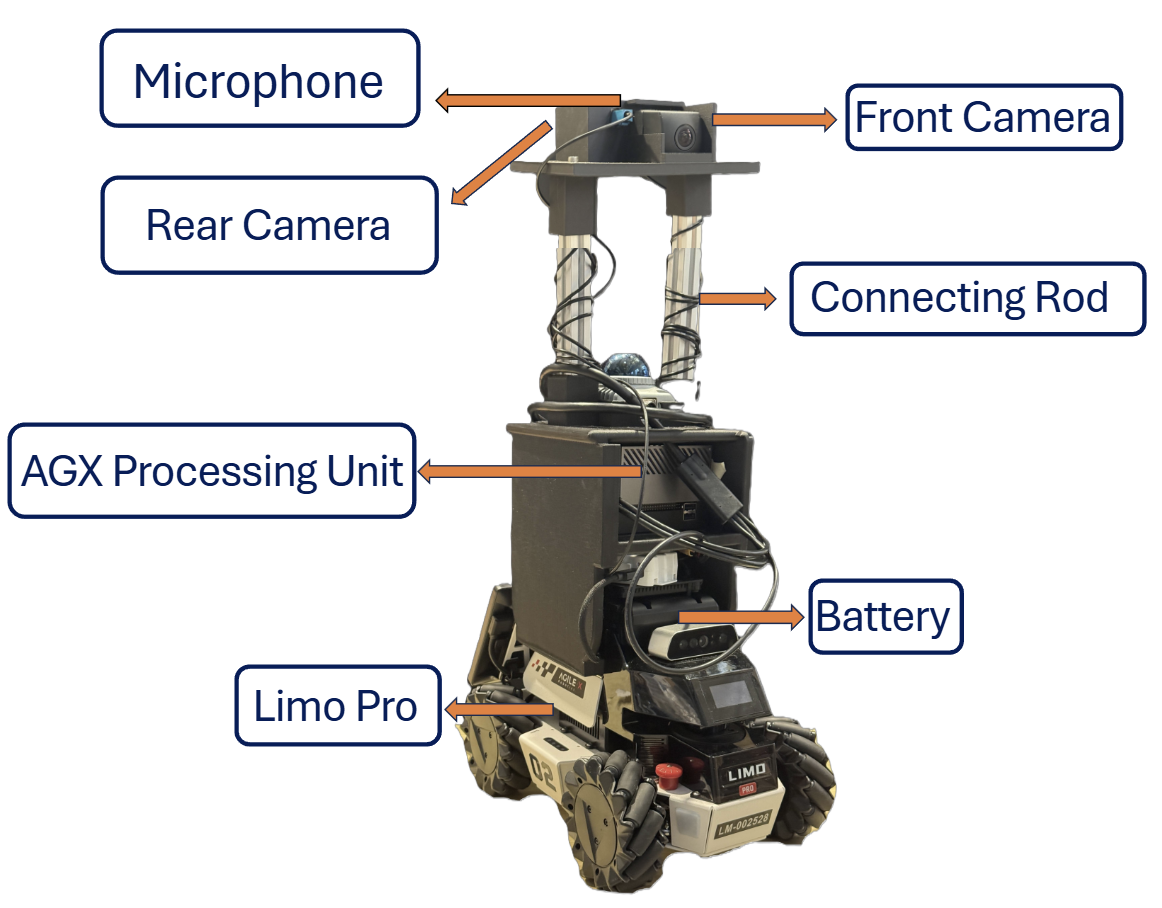
\includegraphics[width=0.9\columnwidth]{figures/setup.png}
    \caption{The robot hardware platform.}
  \end{subfigure}
  
  % reduced vertical spacing
  \vspace{2pt}
  
  % (b) Scene photo
  \begin{subfigure}{0.95\columnwidth}
    \centering
    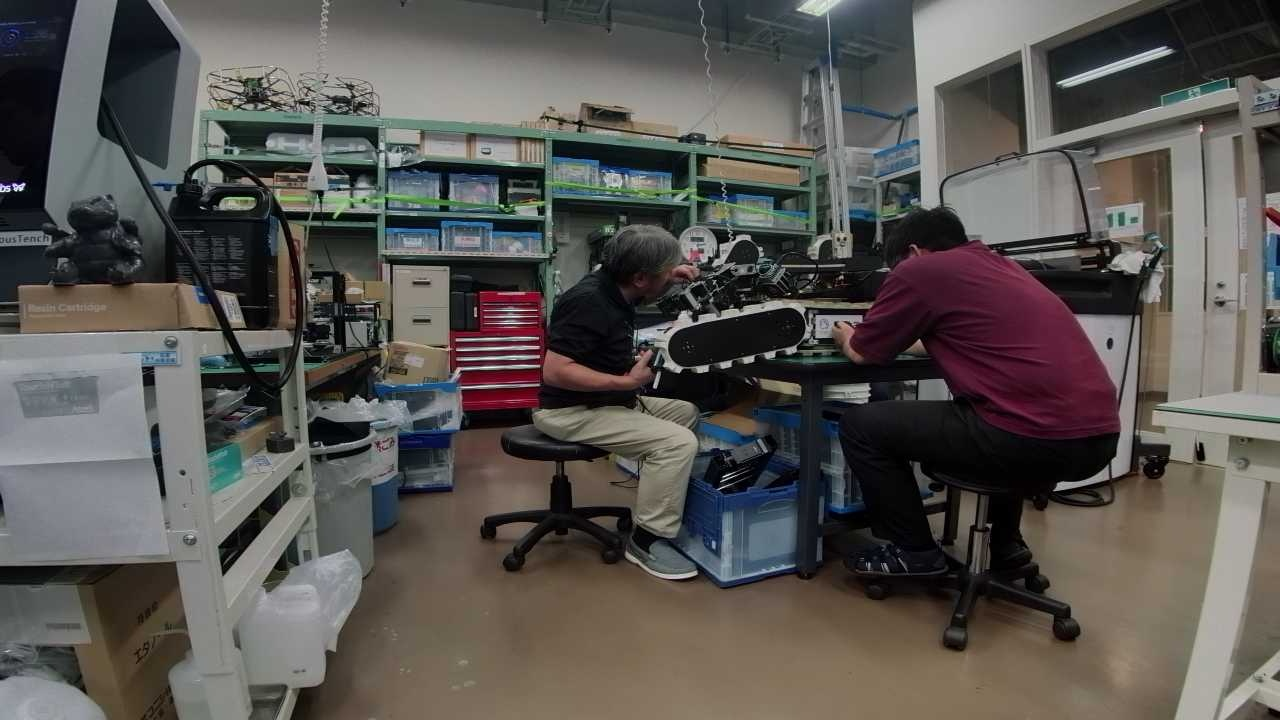
\includegraphics[width=0.9\columnwidth]{figures/scene.jpg}
    \caption{Example scene perception.}
  \end{subfigure}
  
  % reduced vertical spacing
  \vspace{2pt}
  
  % (c) Generated article text box
  \begin{subfigure}{0.95\columnwidth}
    \centering
    \fbox{\parbox{0.9\columnwidth}{\footnotesize
    \textbf{Headline:} New Robot Takes Shape in a University Robotics Workshop\\[2pt]
    \textbf{Article Text:} In a university robotics workshop, two researchers work side-by-side at a central bench, assembling a tracked mobile robot. The robot sits atop the table with its black tread and sensor mounts clearly visible as one researcher adjusts wiring while the other reviews components. Around them, shelves of labeled bins, tools, and test equipment frame the scene, highlighting an active lab environment. The focus remains on the robot under construction, but the organized background underscores ongoing development and the team's hands-on, technical workflow.}}
    \caption{Autonomously generated article.}
  \end{subfigure}
  
  \caption{An overview of our au\-ton\-omous journalism system, showing (a) the mobile platform, (b) a perceived scene, and (c) the final generated article.}
  \label{fig:overview_stack}
\end{figure}



In this paper, we propose a fully au\-ton\-omous journalist robot that tightly couples real\-time data collection with article generation with complete perception to publication pipeline, as illustrated in Fig.~\ref{fig:overview_stack}. The system employs vision–language models for scene understanding and robot control, enabling au\-ton\-omous movement and newsworthi\-ness‑driven data collection from dual cameras that provide 360° coverage. Multi\-modal data are processed via visual analysis and semantic selection, and a language model then synthesizes grounded articles based on synchronized frame descriptions and audio transcripts. Audio–video synchronization ensures factual narratives, and a closed‑loop architecture performs on‑the‑fly evaluation that feeds back into selection and motion policies, operating without human intervention to deliver low‑latency, au\-ton\-omous journalism from sensing to publication.

Our contributions are: (i) newsworthi\-ness‑driven au\-ton\-omous data collection that dynamically controls robot motion and capture decisions to improve positioning and selectivity, with feedback from the journalism process used to refine pose and coverage quality; (ii) a unified, real\-time journalism pipeline that couples data collection with content production to reduce capture‑to‑publication latency; (iii) synchronized, multi\-modal processing that aligns audio–visual evidence and generates grounded jour\-nal\-is\-tic content from frame descriptions and transcripts; and (iv) a comprehensive, multi\-modal evaluation framework with multiple specialized spatial–temporal–semantic metrics, including factual verification, video relevance scoring, and jour\-nal\-is\-tic quality measures not available in existing frameworks.

\section{RELATED WORK}

The related work in au\-ton\-omous journalism robotics can be categorized into three main areas: 

\subsection{Data Processing and News Content Generation}

Data-to-text systems establish the foundation for automated journalism and motivate our focus on integrating collection with generation. Foundational works convert structured data into narrative content \cite{diakopoulos2019automating,graefe2016guide,montana2020automating}, analyzing how rule-based NLG turns financial reports, election results, and sports statistics into articles. Modern implementations process various data sources \cite{reuters_tracer2017,xiaomingbot2020,blab_reporter2022}. However, reliance on pre‑structured sources leaves a disconnect from live collection \cite{diakopoulos2019automating,graefe2016guide}, creating timeliness and adaptability gaps in dynamic news environments.

Multi\-modal generation research frames our use of extractive and abstractive methods for jour\-nal\-is\-tic content. Core approaches include extractive selection of key segments/frames and abstractive narrative generation from multimedia \cite{video_summarization_2024}. Recent multi-modal models \cite{li2024llava,videollama3_2025,blip22023} have advanced visual-language understanding for journalism. While cross‑domain alignment methods \cite{mhms2022} enable better integration, end‑to‑end systems that simultaneously process audio, visual, and textual modalities \cite{li2024llava,videollama3_2025} for jour\-nal\-is\-tic generation remain underexplored. Evaluation frameworks for automated journalism have evolved from basic factuality checks \cite{selfcheckgpt2023,factscore2023} to comprehensive quality assessment \cite{qafacteval2021}.

\subsection{Data Collection}

Data collection methods motivate our fully au\-ton\-omous approach. Traditional journalism relies on human crews for gathering and curating information \cite{pew2021newsroom}, while recent robotics introduce mobile and telepresence systems to capture visual and audio data \cite{adversarial_data_collection_2025,sharedassembly_2025,robots_diary_studies_2025}. Examples include social robots integrated with LLMs for conversational reporting \cite{newsgpt2023}, demonstrating AI‑enhanced reporters. However, most systems remain teleoperated—requiring continuous human supervision and following predefined routes or static setups \cite{adversarial_data_collection_2025,sharedassembly_2025,robots_diary_studies_2025}—which limits scalability and induces operator fatigue and latency. 

\subsection{Robot Embodiment}
Embodiment research underpins our navigation and decision‑making design. Vision-language navigation has progressed in various approaches \cite{duet2022}, while language‑grounded control grounds high‑level semantics into affordance‑aware policies \cite{saycan2022}. Robotics transformers \cite{brohan2022rt} have demonstrated the potential for large-scale language models in robotic control. However, no prior work applies embodied navigation to journalism or implements newsworthi\-ness‑driven navigation, underscoring our novelty: directly coupling editorial newsworthi\-ness with embodied control to guide real\-time data acquisition.
\noindent\textit{Novelty positioning:} Surveys on embodied navigation and multi\-modal navigation \cite{liu2025embodiednav,wu2024embodiedsurvey} do not report systems that couple real\-time, newsworthiness\-driven control with synchronized journalism generation and an autonomous evaluation gate, which motivates our integrated formulation.

\begin{figure*}[!t]
\centering
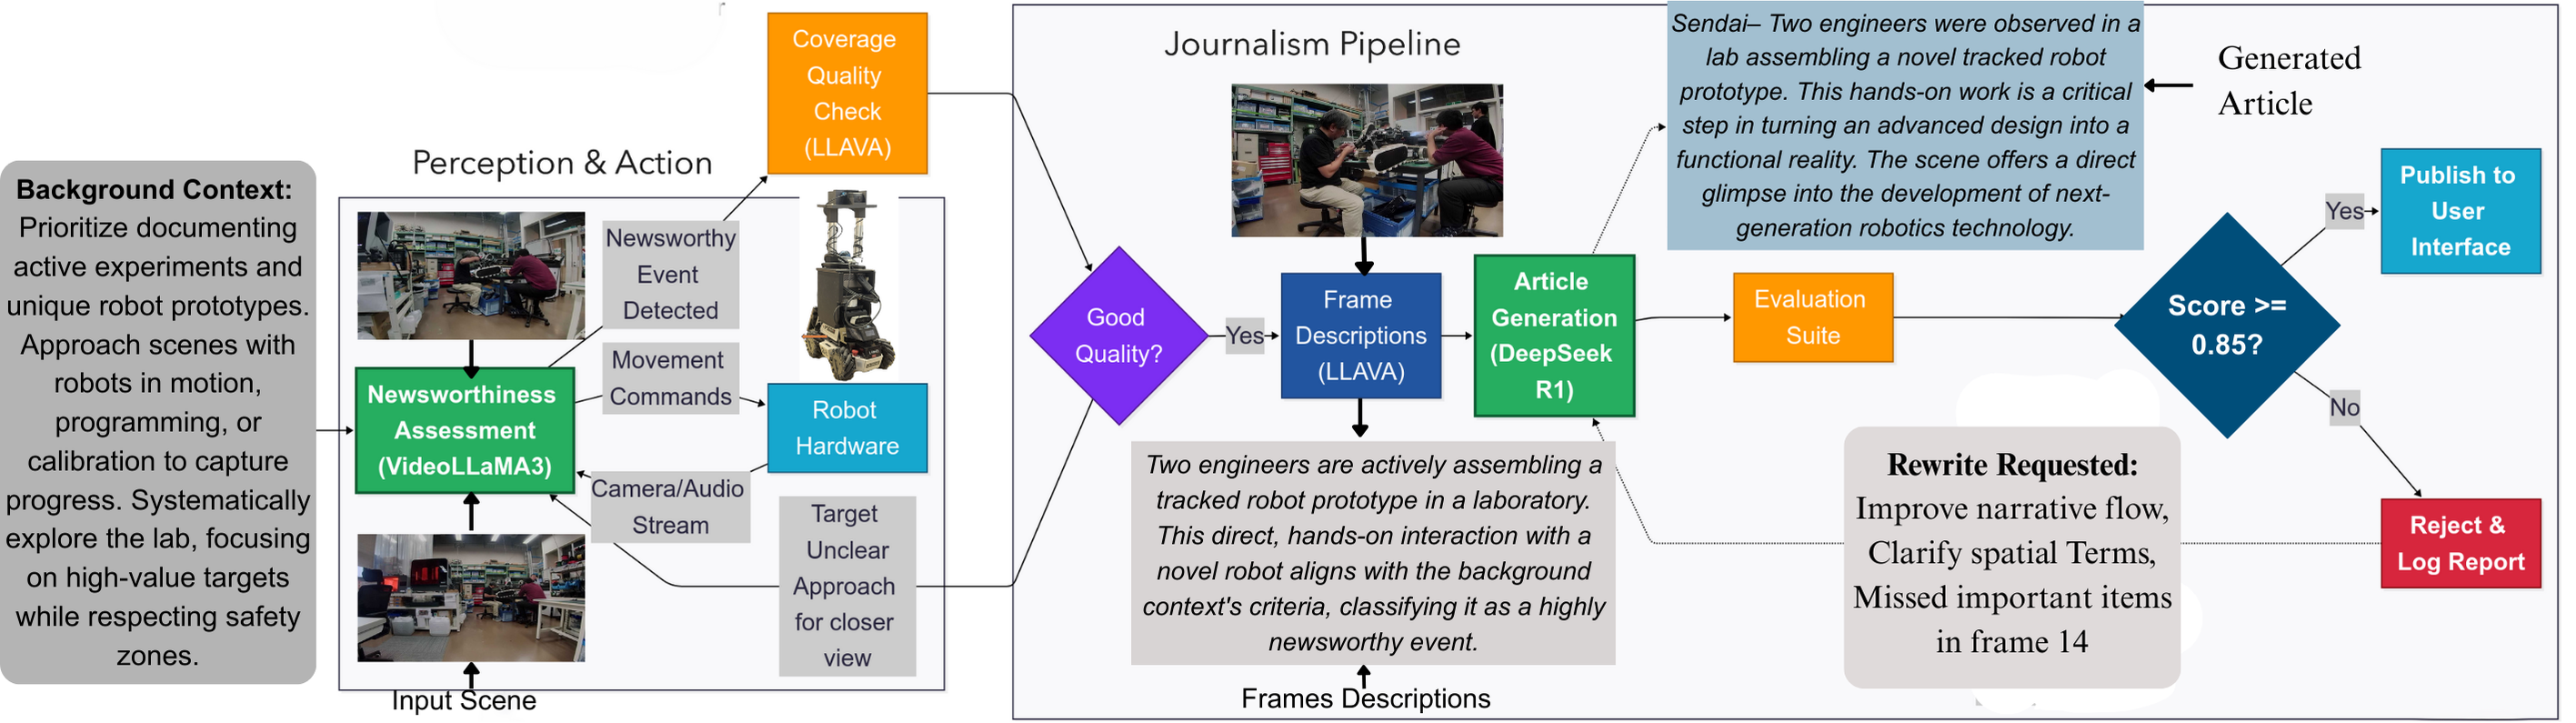
\includegraphics[width=\textwidth]{figures/flowchart.png}
\caption{End-to-end autonomous journalism pipeline with example scene input and outputs. Left: Perception \& Action loop couples mission context to newsworthi\-ness assessment, robot motion, and coverage quality checks, showing example laboratory scene input and robot hardware. Right: Journalism pipeline processes frame descriptions into a draft article, scores it with the evaluation suite, and either publishes (score $\ge 0.85$) or requests a targeted rewrite, with example frame description and generated article output displayed.}
\label{fig:flowchart}
\end{figure*}

Addressing these gaps, our system (1) closes the collection–generation disconnect by coupling capture policy to on‑the‑fly editorial signals, avoiding reliance on pre‑structured inputs and post‑hoc processing \cite{diakopoulos2019automating,graefe2016guide,reuters_tracer2017,xiaomingbot2020,blab_reporter2022}; (2) operates without a human operator dependency using newsworthi\-ness‑driven navigation and synchronized audio–visual capture, easing the human‑in‑the‑loop bottleneck reported in mobile/telepresence data‑collection frameworks \cite{adversarial_data_collection_2025,sharedassembly_2025,robots_diary_studies_2025}; (3) mitigates multi\-modal fusion limits by aligning acquisition with editorial intent during capture rather than relying solely on post‑hoc summarization \cite{mast2020,mhms2022,video_summarization_2024}; and (4) operationalizes embodied navigation for journalism with policy decisions driven by a real‑time newsworthi\-ness score—capabilities absent from prior embodied AI work \cite{embodied_survey_2024,duet2022,saycan2022}. Collectively, this yields an end‑to‑end system that improves coverage quality, reduces capture‑to‑publication latency, and operates without a human operator dependency while producing intent‑aligned outputs.

\section{METHODOLOGY}


We summarize the overall workflow in Fig.~\ref{fig:flowchart}; the following subsections explain these processes.

\subsection{Detection, Perception, and Newsworthiness Assessment}
To extract scenes for journalism, scene recognition is performed by conditioning the base model on mission‑specific background context (a concise brief describing subjects of interest, safety constraints, and editorial priorities), mimicking the workflow of human journalists. Foundation vision–language models (VLMs) such as CLIP \cite{radford2021clip}, Flamingo \cite{alayrac2022flamingo}, LLaVA-Interleave \cite{li2024llava}, VideoLLaMA3 \cite{videollama3_2025}, and BLIP-2 \cite{blip22023} are trained on large, heterogeneous web‑scale corpora, yielding broad, general‑purpose perceptual priors. In unconstrained, dynamic reporting settings, we observed that using these models ``as is'' produces diffuse and temporally inconsistent scene interpretations that are insufficient for reliable editorial decisions. To specialize perception for journalism, we condition the model on a mission‑specific \emph{background context}—a compact brief describing subjects of interest, safety constraints, and editorial priorities—analogous to how human journalists operate. Concretely, we inject this context into the multi\-modal prompt so that perception and subsequent movement choices are explicitly evaluated against newsworthiness criteria rather than generic salience. The prompt uses structured elements—system role, confidence calibration thresholds, and a newsworthiness rubric (relevance to mission, importance/impact, evidence clarity/grounding, novelty, and safety/compliance)—to guide decision reliability; see the excerpt below.

\vspace{-1pt}
\noindent\fbox{\parbox{0.97\columnwidth}{\footnotesize\itshape \emph{Prompt excerpt (controller):} System role: \emph{Intelligent exploratory journalist robot controller}. The mission background (subjects, priorities, safety) is injected verbatim; all decisions must be grounded in the current video and the brief. \emph{Confidence calibration}: high (0.8--1.0), medium (0.6--0.8), low (0.4--0.6), very low (0.0--0.4) $\Rightarrow$ speed/safety scaling. \emph{Vision-first rules}: forward 0.6--0.8 m/s when targets/open path are visible; rotation 1.2--2.0 rad/s for scanning/reframing. \emph{Safety}: never move forward if the center path appears blocked; maintain distance; use conservative speeds at low confidence. \emph{Output instruction}: return concise natural-language reasoning and the movement commands (\texttt{linear\_x}, \texttt{angular\_z}) with a confidence value; omit any other text.}}

To enable responsive control in dynamic scenes, we segment real\-time video into short (\(\sim\!2\,\text{s}\)) windows, which shortens the perception–action cycle and mitigates VideoLLaMA3's non–real\-time‑optimized architecture \cite{videollama3_2025}. Each window is then evaluated using: (i) the dynamic background context that can be updated externally, (ii) a stable instruction‑following prompt (see the prompt excerpt box) that defines the output schema and robot control interface, and (iii) a concise summary of recent commands to reduce repetition and encourage exploratory coverage. VideoLLaMA3 \cite{videollama3_2025} processes this combined input and returns a single, structured response that couples natural‑language reasoning describing the scene and its relevance to the background context with a movement proposal, a newsworthi\-ness score, a confidence score, and an explicit start/continue/stop trigger for recording and journalism pipeline activation \cite{videollama3_2025}. Once the journalism pipeline is started, the robot continues exploratory navigation while awaiting feedback on captured data quality and any movement adjustments recommended by the journalism process to improve coverage.


\textbf{Newsworthiness and control:} We smooth the model's per‑window newsworthi\-ness estimate and form an overall score $N_t$ as a weighted sum of three signals: smoothed newsworthi\-ness, agreement with the mission brief, and optional novelty (weights sum to 1). Recording begins when $N_t \ge 0.7$ and confidence $c_t \ge 0.8$ and stops when both drop below 0.3 and 0.5, respectively (hysteresis). Motion is tied to $N_t$ and path clearance: when the path is clear and $N_t$ is high the robot moves forward; otherwise it rotates to reframe, with speeds scaled down under low confidence. Safety reflexes (obstruction turns), hysteresis, and emergency stops are always active. Decision policy: start the journalism pipeline when $N_t \ge \tau_w$ and $c_t \ge \tau_c$ with $\tau_w{=}0.7$ and $\tau_c{=}0.8$; stop when $N_t{<}0.3$ and $c_t{<}0.5$. Let $F_t\in\{0,1\}$ indicate a clear forward path and $d_t\in\{-1,+1\}$ the preferred turn direction. The commanded velocities are
\[ v^{\text{lin}}_t = v_{\max} N_t F_t,\quad v^{\text{ang}}_t = \omega_{\max} (1{-}N_t) (1{-}F_t) d_t, \]
optionally scaled by confidence, $ (v^{\text{lin}}_t, v^{\text{ang}}_t) \leftarrow \sigma(c_t) (v^{\text{lin}}_t, v^{\text{ang}}_t)$ with $\sigma(c)\in\{0.4,0.6,0.8,1.0\}$. The journalism pipeline is triggered only during high‑$N_t$ segments so that processed evidence aligns with key moments.

\textbf{Rationale and sensitivity:} Thresholds $\tau_w{=}0.7$ and $\tau_c{=}0.8$ were selected via a small validation sweep ($\tau_w\in\{0.6,0.7,0.8\},\,\tau_c\in\{0.7,0.8,0.9\}$) on held‑out runs to balance false starts (off‑brief/low‑confidence recording) against missed opportunities. Settings lower than 0.7/0.8 increased off‑topic segments; higher values reduced recall of fleeting events.

\subsection{Journalism Pipeline: Multimodal Data Processing and Content Generation}
Once a newsworthi\-ness event is triggered, the journalist pipeline begins continuous real\-time monitoring of the combined dual-camera feed (front + rear, providing 360° coverage) together with the live audio stream, and prepends a \(\sim\!10\,\text{s}\) pre-event context window to preserve environmental history. The 10\,s horizon was chosen as a practical compromise observed in pilot runs: shorter windows ($<5\,s$) omitted setup cues relevant to our scenarios (e.g., subject handovers, equipment operation), while much longer windows increased latency and evidence-retrieval cost without added benefits; 10\,s matched the typical utterance/shot-change scale we encountered. The first step is a fast quality and relevance check using a vision–language model (LLaVA) \cite{liu2023llava, li2024llava}. If the captured view is unclear, off-topic, or poorly framed, the pipeline issues structured feedback to the perception and newsworthi\-ness loop with actionable guidance (e.g., rotate toward the subject, adjust distance/centering) to improve coverage before continued recording. If the data quality is sufficient, the pipeline proceeds as follows.

\textbf{Semantic selection:} Visual redundancy is reduced via semantic selection using CLIP (ViT-B/32) \cite{radford2021clip} to retain frames that best represent salient scene changes while discarding near‑duplicates. This extractive step reduces processing time without sacrificing coverage quality by preserving the information needed for abstractive generation, consistent with extractive/abstractive video summarization practice \cite{video_summarization_2024}. Selected frames are grouped into compact batches to preserve short‑range temporal coherence. Table~\ref{tab:selection_efficiency} summarizes typical reduction and processing effects over three representative runs.

\begin{table}[!h]
\centering
\caption{Effect of Semantic Selection on Processing (N=6, averages; averaged over 6 runs per row). Note: processing time is the full pipeline segment to produce frame descriptions; selection uses CLIP (ViT-B/32) with an 87\% similarity threshold and a short dedup window to suppress redundant frames, tuned empirically to track scene changes.}
\label{tab:selection_efficiency}
\scriptsize
\begin{tabularx}{\columnwidth}{|>{\raggedright\arraybackslash}X|c|c|>{\raggedright\arraybackslash}X|}
\hline
 \textbf{Experiment} & \textbf{Total Frames} & \textbf{Selected Frames} & \textbf{Processing Time (s)} \\
\hline
 Lab: Empty Desks & 2500 & 600 & 136 (vs 294 w/o selection) \\
\hline
 Lecture: Screen+Board & 2500 & 480 & 128 (vs 286 w/o selection) \\
\hline
 Workshop: Equipment & 2500 & 410 & 122 (vs 272 w/o selection) \\
\hline
\end{tabularx}
\end{table}

\vspace{-3pt}
\textbf{Multi\-modal description:} For each batch of 8 frames, a multi\-modal VLM (LLaVA–NeXT–Interleave) \cite{li2024llava} produces concise, time‑ordered visual descriptions grounded in the background context \cite{li2024llava}, while the audio stream is transcribed by automatic speech recognition (Whisper) \cite{whisper2022} and aligned on the same timeline. The resulting text units (visual descriptions and speech transcripts) are synchronized so that auditory events and visual observations are associated with the correct moments.
To maintain a consistent narrative and improve temporal understanding, each new batch is processed together with the immediately preceding batch's visual descriptions and speech transcripts, reducing hallucination and strengthening scene and environment continuity across batches.

\textbf{Real\-time processing architecture:} Frame descriptions are generated continuously in the background during data collection, enabling immediate article generation upon mission completion. This parallel processing approach ensures real\-time responsiveness while collecting data, with frame descriptions produced asynchronously as new footage is captured. Article generation begins immediately after data collection ends, with completion times depending on content complexity, the volume of collected data, and semantic selection processing (Table~\ref{tab:selection_efficiency}).

\textbf{Prompted synthesis and grounding:} For article generation, the pipeline constructs a structured prompt with (i) the mission background context, (ii) the synchronized visual descriptions and transcripts, and (iii) a brief timeline of key events. A retrieval‑augmented grounding step indexes the accumulated descriptions/transcripts to ensure that generation cites the most relevant evidence and so that information can be efficiently retrieved later to answer detailed queries. These grounded inputs are then synthesized by a reasoning‑augmented language model (DeepSeek‑R1) \cite{deepseekai2025deepseekr1incentivizingreasoningcapability} using a structured prompt that explicitly binds evidence segments to the requested headline, lead, and body, yielding a long‑form article that follows the inverted‑pyramid structure—leading with the most newsworthy information before elaborating supporting details \cite{herrero2024circular}. The article is output in text and audio formats and is then passed to the evaluation algorithms; the system awaits feedback to guide any further refinements.

\subsection{Evaluation and Acceptance}
Given an article draft with synchronized frame descriptions, selected keyframes, and the audio transcript, the evaluation framework runs as a separate process and scores outputs across the defined dimensions; the metrics and signals are summarized in the Evaluation Dimensions table II.

\begin{table}[!h]
\centering
\caption{Evaluation Dimensions and Models}
\label{tab:eval_summary}
\scriptsize
\setlength{\tabcolsep}{3pt}
\begin{tabular}{|l|p{2.1cm}|p{2.05cm}|}
\hline
\textbf{Dim.} & \textbf{Purpose} & \textbf{Model/Signal} \\
\hline
Visual–Text Rel. & Evidence–text match & CLIP sim./retrieval \\
\hline
Multimodal Fact. & Grounding; claim entailment & BLIP/VQA; RoBERTa--MNLI \\
\hline
Sem./Temp./Spat. Consistency & Across frames + descriptions & LLaVA-Interleave eval. \\
\hline
Language Quality & Coherence; grammar/style; structure & SBERT; LanguageTool; structure \\
\hline
\end{tabular}
\end{table}

\noindent\textbf{Evaluation framework:} The evaluation process aggregates complementary signals to gate acceptance. Article sentences are embedded with Sentence‑BERT \cite{reimers2019sentencebert} to measure intra‑article coherence; keyframes and batch descriptions are scored for semantic/visual/temporal agreement via LLaVA-Interleave \cite{li2024llava}; claim–evidence pairs are tested with RoBERTa‑MNLI \cite{liu2019roberta}; and CLIP \cite{radford2021clip} provides sentence–frame relevance and retrieval‑style recall. We compute an overall score as and average of the evaluation dimensions (Rel., Fact., Consistency, Language, Video). Decision policy: Across multiple experiments, outputs with $S>0.85$ were consistently publishable—factually accurate, grounded in evidence, and stylistically acceptable—while packages below this level typically required revision. If the overall score is less than 0.85 across the active metrics, the system routes the package back to article generation with a structured evaluation report; otherwise ($\ge 0.85$), the article is accepted post‑evaluation and grounding for publication. This autonomous gate, driven by multiple metrics, improves and controls the quality of generated content and is central to achieving full autonomy—removing dependence on limited human evaluation resources; Table~\ref{tab:article_quality} reflects its impact on acceptance outcomes.

Upon acceptance, the article is served through a chat interface backed by retrieval‑augmented generation over the recorded evidence.

\section{Experimental and Evaluation Setup}

\subsection{Hardware Setup}
As illustrated in Fig.~\ref{fig:overview_stack}(a), we mount dual cameras for 360° visual coverage and a microphone array for spatial audio cues. All sensors connect to an on‑board processing unit (AGX Orin) that handles data ingest and streams to a remote GPU server for perception and content generation. Motion is executed by a mobile base that receives velocity commands over ROS~2.

On‑board nodes handle sensing and motion I/O, while a remote NVIDIA A100 GPU runs perception and journalism processing. End‑to‑end control latency is 130–170~ms over campus Wi‑Fi, enabling real‑time navigation decisions, while article‑pipeline latency scales with selected frames (Table~\ref{tab:selection_efficiency}). Custom enclosures organize the system with a sensor mast to approximate person‑eye viewpoint and reduce occlusions in crowded scenes.



\subsection{Experiments and Evaluation}
We evaluate the system across three stages: navigation control, article generation quality, and end-to-end integration. The following subsections detail the experimental setups.

\subsubsection{Newsworthiness-Driven Navigation}
\textit{Hypothesis:} adding mission context and journalism feedback increases alignment with a human operator and improves coverage quality under identical budgets.
We evaluate navigation across three environments (Research Lab, Research Workshop, Lecture Room) using four approaches. \emph{Procedure}: each run executes a fixed budget of 70 movement decisions; a "movement decision" is one discrete control proposal from the \(~2\,\text{s}\) newsworthi\-ness window that, after safety gating, issues a forward or turn command. \emph{Metrics}: (1) decision alignment with the human baseline (percentage of executed actions that match the human's forward/turn choice at the same decision index), (2) coverage quality (percentage of time with a clear view of the scene subject), (3) total distance traveled (meters), (4) runtime (total time to complete 70 movement decisions). \emph{Human‑operator comparison}: in each environment we run four experiments under identical conditions: (1) Teleoperation baseline—a human operator drives the robot to collect data and all movement is recorded; (2) Autonomous without background—the controller runs using only a generic journalist‑role prompt, without a mission background context; (3) Autonomous with background only—the controller is conditioned on a mission‑specific background context; (4) Autonomous with background and journalism feedback—the controller also receives coverage feedback from the journalist pipeline. We then compare the movement decisions across these experiments to assess alignment with the human operator. Results: Table~\ref{tab:navigation_comparison}.

\subsubsection{Effect of Background-Context Variation on Navigational Decisions}
\textit{Hypothesis:} changing the background context alone induces substantially different navigation choices in the same environment.
We repeat au\-ton\-omous runs in the same environment and setting with two different background contexts, and replicate this pair across three different environments. This isolates how the mission brief steers perception and movement choices under otherwise identical conditions. Results: Table~\ref{tab:behavioral_divergence} and Fig.~\ref{fig:context_variation}.

\subsubsection{Single-Frame vs. Multi-Frame Processing}
\textit{Hypothesis:} multi‑frame visual processing yields higher temporal consistency and spatial reasoning than single‑frame baselines.
Initially, we used a single‑frame generator (Llama 3.2 \cite{llama3_2024}), which accepts one frame at a time; timelines and cross‑frame relevance were harder to maintain and sometimes yielded brittle descriptions. We then switched to an LLaVA‑based formulation \cite{liu2023llava,li2024llava} that accepts multiple frames per query \cite{liu2023llava,li2024llava}. We tested both approaches in the same settings and evaluated outputs with the above algorithm to measure the effectiveness of multi‑frame processing. Results: Table~\ref{tab:single_vs_multiframe}.

\subsubsection{Generated Article Quality: End-to-End System Evaluation}
\textit{Hypothesis:} newsworthiness‑driven autonomous collection improves overall article quality relative to static recorded data.
We conduct experiments with different scenarios in three environments and, using the previously described evaluation algorithm, assess the generated articles to measure overall quality. To evaluate the functionality and effectiveness of the full system, we test end‑to‑end processing and article creation using recorded data and the newsworthi\-ness‑driven navigation approach in the same environment settings. This assesses how effectively the feedback loop between journalism generation and newsworthi\-ness assessment improves coverage quality and clarity, capturing important events without missing key scenes or producing low‑quality footage. Results: Table~\ref{tab:article_quality}.

\vspace{-2pt}
\section{RESULTS}

We report results that (i) reduce reliance on teleoperation under the same 70-decision budget, (ii) demonstrate synchronized multi\-modal processing benefits via multi-frame evaluation, and (iii) close the collection–generation disconnect through an acceptance gate at $S\!\ge\!0.85$; procedures follow Section IV-B.

\subsection{Newsworthiness-Driven Navigation}

The aggregated comparison across the four approaches under a fixed budget of 70 decisions is presented in Table~\ref{tab:navigation_comparison}. Bridging collection and generation via background context and journalism feedback yields alignment and coverage that closely match the teleoperated baseline, while removing the need for a human operator during capture.

\begin{table}[!h]
\centering
\caption{Multi‑Metric Performance Comparison of Navigation Controllers (N=3, averages). Alignment is the match of movement decisions with the human operator at the same decision index; Coverage is the fraction of time the subject is clearly in view. Runtime is total time to complete 70 decisions.}
\label{tab:navigation_comparison}
{\scriptsize
\setlength{\tabcolsep}{3pt}
\begin{tabular}{|l|c|c|c|c|c|}
\hline
\textbf{Approach} & \textbf{Total} & \textbf{\shortstack{Aligned\\(\%)}} & \textbf{\shortstack{Coverage\\(\%)}} & \textbf{\shortstack{Dist.\\(m)}} & \textbf{\shortstack{Run\\time}} \\
\hline
Human Operator & 70 & 100\% & 95\% & 15.2 & 2:13 min \\
Generic Prompt & 70 & 42\% & 38\% & 21.5 & 5:27 min \\
With Context & 70 & 82\% & 85\% & 16.5 & 2:54 min \\
Context + Feedback & 70 & 94\% & 93\% & 15.5 & 3:11 min \\
\hline
\end{tabular}
}
\end{table}

For a fixed budget of 70 decisions, the generic‑prompt controller aligned with the human operator on 42\% of decisions (N=3, average); conditioning on background context increased alignment to 82\% and adding journalism feedback yielded 94\% with 93\% coverage quality; both improvements vs. Generic were significant on paired tests. Under identical budgets, these paired results approach teleoperated behavior in alignment and runtime while removing continuous human control during capture. This explicitly shows that bridging collection and generation (via background context and feedback) improves coverage and decision quality in situ, not only post hoc.

\subsection{Effect of Background-Context Variation on Navigational Decisions}

As defined in Section~IV‑B, we assess Behavioral Divergence (\%) between two au\-ton\-omous runs per environment using distinct mission briefs (70 decisions per run). Results are in Table~\ref{tab:behavioral_divergence}, with a qualitative example in Fig.~\ref{fig:context_variation}.

\begin{table}[!h]
\centering
\caption{Analysis of Behavioral Divergence. Note: divergence is measured as the fraction of differing movement decisions over 70 indexed decisions.}
\label{tab:behavioral_divergence}
\scriptsize
\setlength{\tabcolsep}{2pt}
\begin{tabular}{|P{1.55cm}|P{1.15cm}|P{1.15cm}|c|c|c|}
\hline
\textbf{Environment} & \textbf{Context A} & \textbf{Context B} & \textbf{Shared} & \textbf{Divergent} & \textbf{Divergence} \\
 &  &  & \textbf{(70)} & \textbf{(70)} & \textbf{(\%)} \\
\hline
Research Lab & Focus on People Working & Focus on Empty Desks & 7 & 63 & 90\% \\
\hline
Research Workshop & Capture Robotics Advancements & Focus on Industrial Equipment & 10 & 60 & 86\% \\
\hline
Lecture Room & Focus on Screen and Board & Focus on the Presenter & 6 & 64 & 91\% \\
\hline
\end{tabular}
\end{table}

The data presented in Table~\ref{tab:behavioral_divergence} shows a high degree of behavioral divergence in all tested environments when the mission context was altered. The average divergence across the three scenarios was 89\%. In the Lecture Room experiment, a comparison between the two runs revealed that only 6 of the 70 movement decisions were shared, corresponding to a 91\% divergence in navigational strategy. Similarly, the Research Lab and Research Workshop environments showed high divergence rates of 90\% and 86\%, respectively.

\subsection{Single-Frame vs. Multi-Frame Processing}

The single‑frame baseline (Llama~3.2) \cite{llama3_2024} processes each piece of visual evidence in isolation, while the multi‑frame model (LLaVA-Interleave) \cite{li2024llava} can reason across a sequence of images. We expected this to improve narrative and temporal consistency. Table~\ref{tab:single_vs_multiframe} presents paired results (N=3): the multi‑frame approach achieved a higher Overall Score +23.3\%, with the largest gains in Temporal Consistency (+55.2\%) and Spatial Reasoning (+35.4\%). These gains reflect the benefits of synchronized multi‑modal processing: aligning acquisition and reasoning across frames and transcript context improves cross-frame coherence.

\begin{table}[!h]
\centering
\caption{Evaluation of Single‑Frame vs. Multi‑Frame Approaches (N=3, paired on the same inputs). Paired tests for Overall, Temporal, and Spatial are reported in the text.}
\label{tab:single_vs_multiframe}
\scriptsize
\begin{tabularx}{\columnwidth}{|>{\raggedright\arraybackslash}X|c|c|c|}
\hline
\textbf{Evaluation Metric} & \textbf{\shortstack{Single‑Frame\\(Llama 3.2)}} & \textbf{\shortstack{Multi‑Frame\\(LLaVA)}} & \textbf{\shortstack{Performance\\Gain}} \\
\hline
 Multimodal Factuality & 0.75 & 0.89 & +18.7\% \\
\hline
 Semantic Alignment & 0.80 & 0.91 & +13.8\% \\
\hline
 Spatial Reasoning & 0.65 & 0.88 & +35.4\% \\
\hline
 Temporal Consistency & 0.58 & 0.90 & +55.2\% \\
\hline
 Evidence Quality & 0.78 & 0.89 & +14.1\% \\
\hline
 Video Relevance & 0.77 & 0.87 & +13.0\% \\
\hline
 Overall Score & 0.722 & 0.890 & +23.3\% \\
\hline
\end{tabularx}
\end{table}

\subsection{Generated Article Quality: End-to-End System Evaluation}
\vspace{-3pt}

We compare two data‑collection modalities across three scenarios (Table~\ref{tab:article_quality}). The 'After Eval.' column reports post‑revision scores: packages with Overall \(<0.85\) are returned and re‑evaluated; accepted meet \(\ge 0.85\). Across 12 experiments, the autonomous modality averaged 88\% acceptance vs. 73\% for static and, with near real‑time generation (15.2–24.8 s), closes the capture‑to‑publication loop, operates without a human operator dependency, and improves coverage fidelity (Coverage\% and Evidence Quality) and overall quality. In all three experiments, autonomous outperformed static; Overall rose from 0.734 to 0.861 on average, with per‑scenario gains of 0.780$\to$0.872 (People Working), 0.718$\to$0.848 (Presenter), and 0.705$\to$0.862 (Robotics).

\begin{table*}[!t]
\centering
\caption{Comparative Evaluation of Article Quality (Static Recorded Data vs. Full Autonomous System). N=3 paired runs per scenario (same scenes). Paired tests on Overall per scenario and averaged are reported in the text.}
\label{tab:article_quality}
\footnotesize
\setlength{\tabcolsep}{4pt}
\begin{tabular}{|l|c|c|c|c|c|c|c|c|c|}
\hline
\textbf{Scenario} & \textbf{Modality} & \textbf{Multimodal} & \textbf{Semantic} & \textbf{Spatial} & \textbf{Temporal} & \textbf{Evidence} & \textbf{Video} & \textbf{Overall} & \textbf{After Eval.} \\
 &  & \textbf{Factuality} & \textbf{Alignment} & \textbf{Reasoning} & \textbf{Consistency} & \textbf{Quality} & \textbf{Relevance} & \textbf{Score} & \textbf{(\(\ge 0.85\))} \\
\hline
Lab: People Working & Static Recorded & 0.80 & 0.82 & 0.75 & 0.74 & 0.79 & 0.78 & 0.780 & 0.857 \\
\hline
 & Autonomous & 0.89 & 0.90 & 0.85 & 0.84 & 0.88 & 0.87 & 0.872 & 0.872 \\
\hline
Lecture: Presenter & Static Recorded & 0.74 & 0.76 & 0.69 & 0.68 & 0.72 & 0.72 & 0.718 & 0.854 \\
\hline
 & Autonomous & 0.87 & 0.89 & 0.83 & 0.82 & 0.86 & 0.82 & 0.848 & 0.856 \\
\hline
Workshop: Robotics & Static Recorded & 0.73 & 0.74 & 0.68 & 0.67 & 0.71 & 0.70 & 0.705 & 0.851 \\
\hline
 & Autonomous & 0.89 & 0.90 & 0.83 & 0.84 & 0.87 & 0.84 & 0.862 & 0.862 \\
\hline
Average Score & Static Recorded & 0.757 & 0.773 & 0.707 & 0.697 & 0.740 & 0.733 & 0.734 & 0.854 \\
\hline
 & Autonomous & 0.883 & 0.897 & 0.837 & 0.833 & 0.870 & 0.843 & 0.861 & 0.863 \\
\hline
\end{tabular}
\end{table*}



\textbf{Real\-time performance.} The au\-ton\-omous system demonstrates consistent near real\-time article generation capabilities, with completion times ranging from 15.2 to 24.8 seconds (average: 19.7 seconds) for a set of 7-minute data-collection sessions. These timing measurements represent the duration between the end of the data collection process and the completion of article generation output. This performance is achieved through parallel processing architecture where frame descriptions are generated continuously during data collection, enabling immediate article synthesis upon mission completion. Semantic selection incurs no measurable latency, while frame description generation for each batch of 8 frames takes ~4 seconds on average and runs in the background parallel to data collection. The system operates in two phases: real\-time newsworthi\-ness assessment and navigation (0.5–2 seconds per decision) during data collection, and near real\-time article generation (15.2–24.8 seconds) after collection ends. With mission background context, the robot adapts across diverse indoor environments without environment\-specific retraining, supporting deployment to varied events and mitigating event–reporter mismatches, delays, and undercoverage; the same platform can be specialized per assignment by swapping the brief.

\begin{figure}[!t]
\centering
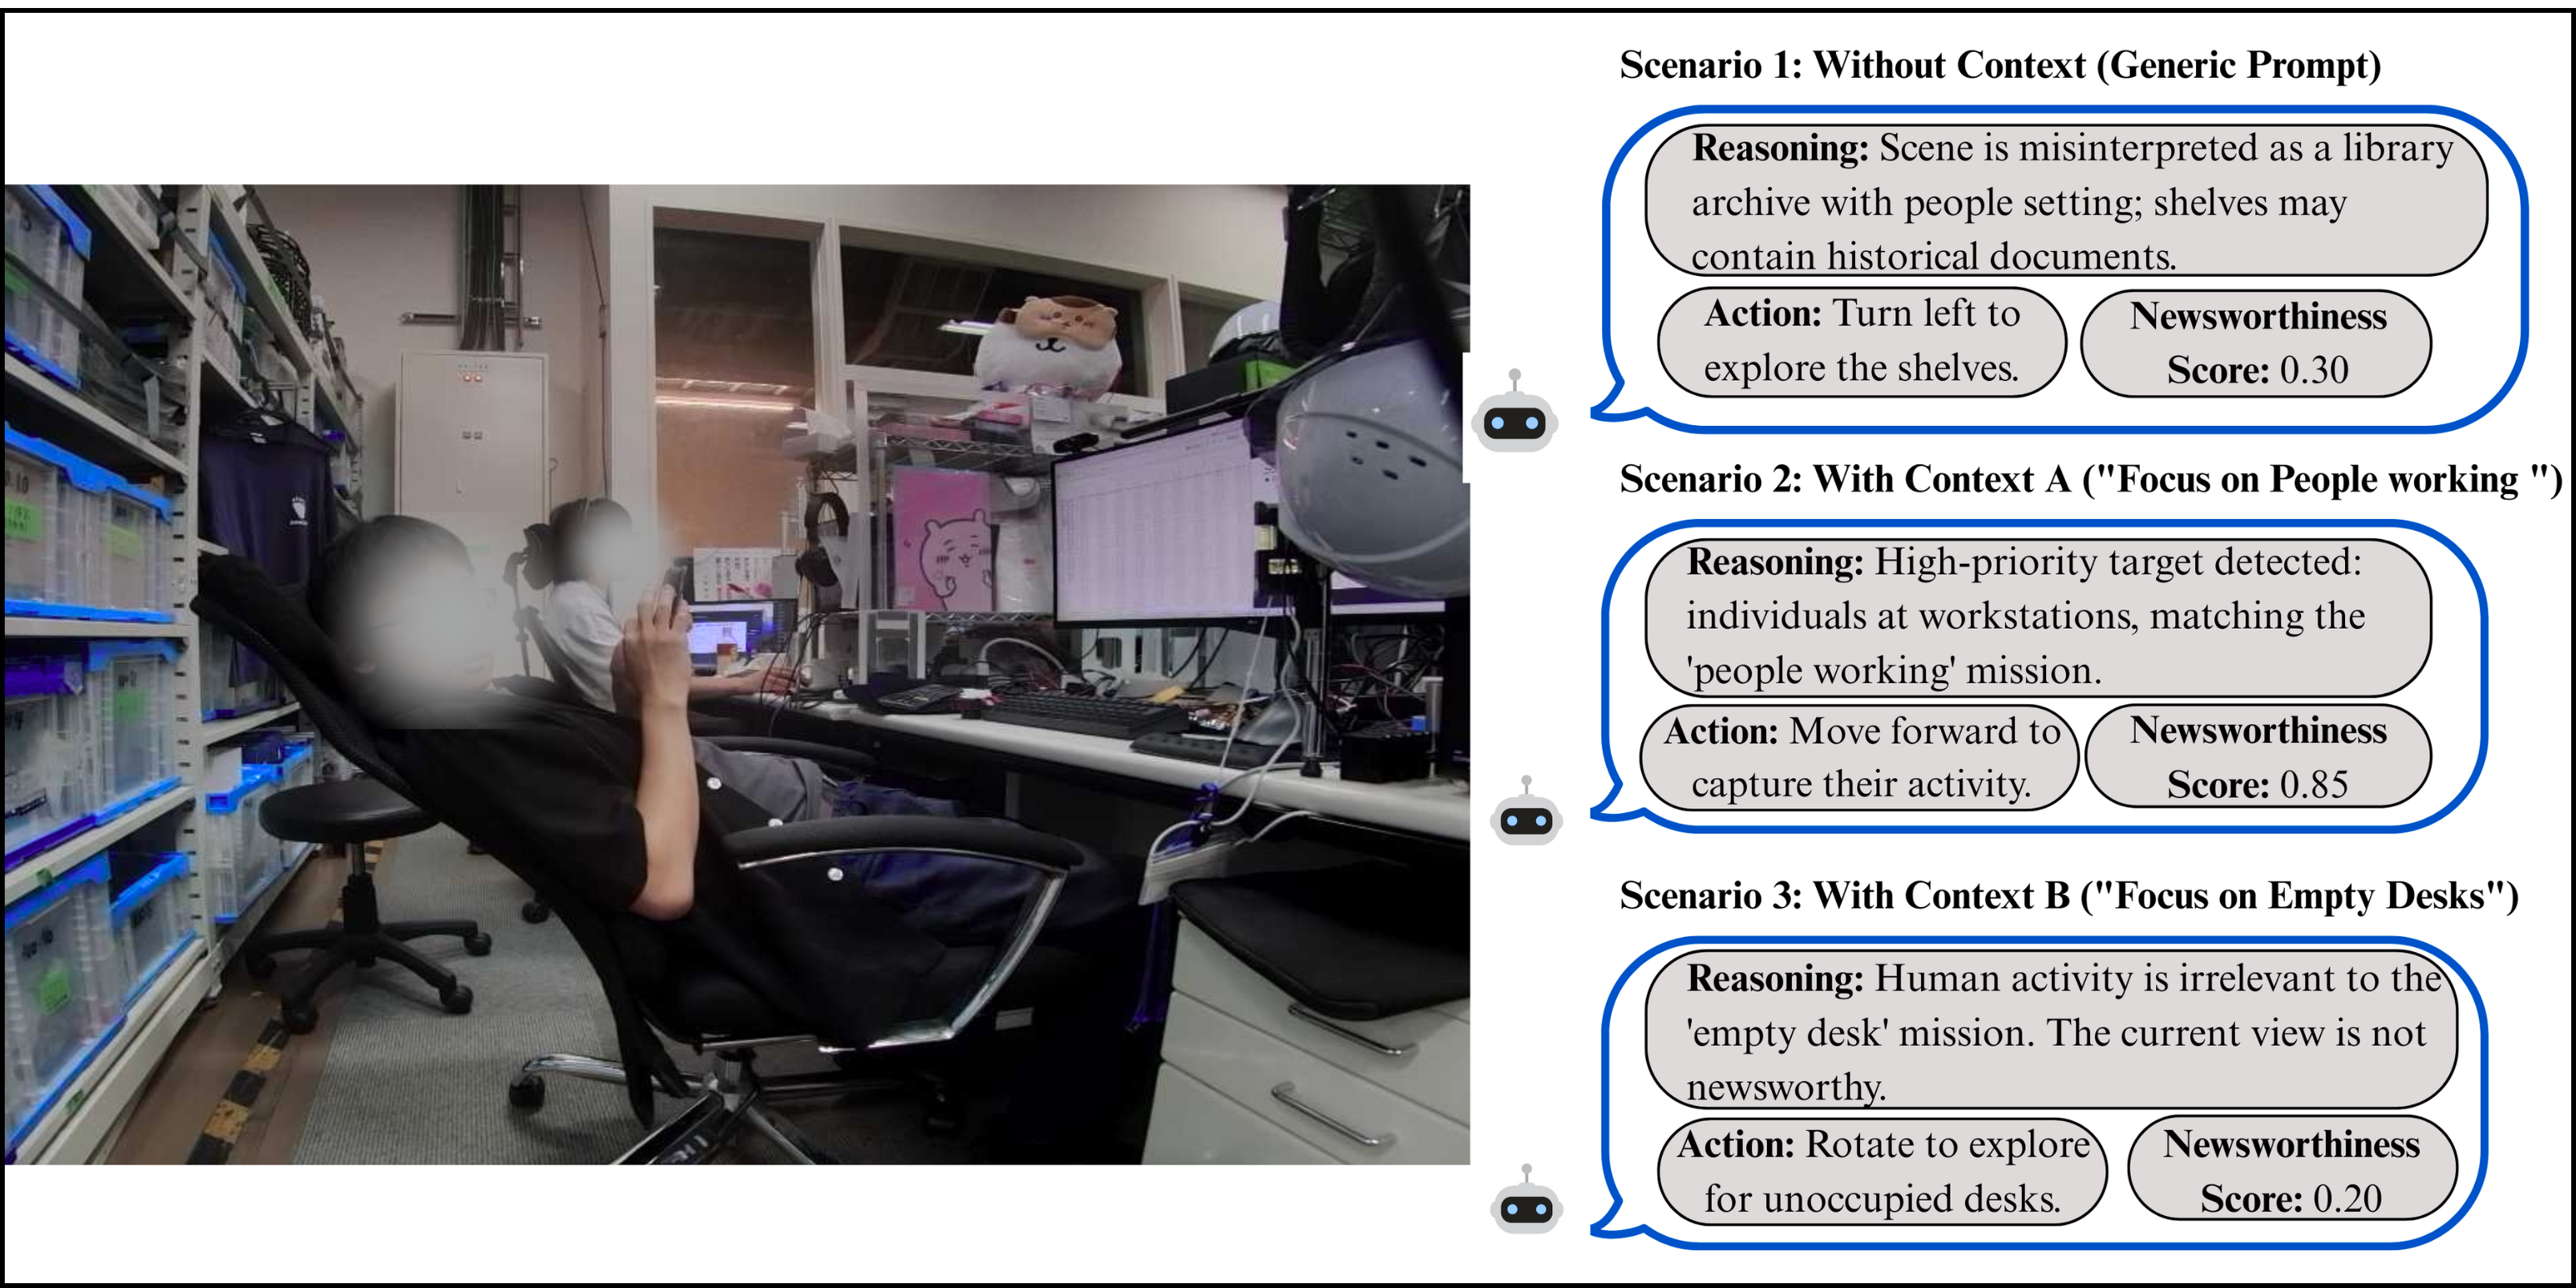
\includegraphics[width=0.96\columnwidth]{figures/editing.png}
\caption{Qualitative example of mission‑context divergence; see Table~\ref{tab:behavioral_divergence}. Divergence is computed as the fraction of differing movement decisions over 70 indexed decisions.}
\label{fig:context_variation}
\end{figure}



\section{DISCUSSION}

\subsection{Role of Context and Feedback in Navigation}

Our experiments (Table~\ref{tab:navigation_comparison}) show how the closed loop reduces reliance on teleoperation and improves coverage: adding mission context raises alignment from 42\% to 82\%, and adding feedback reaches 94\% with 93\% coverage, at near‑human runtimes. Context‑variation tests (Table~\ref{tab:behavioral_divergence}) confirm that the brief steers behavior (\(\sim\!89\%\) divergence). This navigation–journalism feedback loop operationalizes intent during collection, directly addressing the collection–generation disconnect without the need of an operator and improving coverage fidelity.

Runtime analysis reveals the efficiency implications of contextual guidance. The human operator completed the 70-decision sequence in 2:13 minutes, demonstrating optimal decision-making speed. The generic prompt controller required 5:27 minutes, nearly 2.5× longer, as the robot struggled with decision-making and remained static for extended periods without clear guidance. The context-only approach reduced runtime to 2:54 minutes, approaching human efficiency by providing clear mission objectives. The context + feedback approach took 3:11 minutes, approaching human efficiency but slightly longer than context-only due to the additional feedback loop between newsworthiness assessment and the journalism pipeline.

\subsection{The Necessity of Multi-Frame Processing for Coherent Narratives}

The comparative evaluation of single‑frame versus multi‑frame processing (Table~\ref{tab:single_vs_multiframe}) provides a clear justification for our architectural choice. The single‑frame model (Llama 3.2) \cite{llama3_2024}, despite its power, struggled to create narratives, as evidenced by its particularly low scores in Temporal Consistency (0.58) and Spatial Reasoning (0.65). It perceives the world as a series of disconnected snapshots.

The multi-frame LLaVA-based model \cite{li2024llava}, in contrast, demonstrated an improved ability to understand the flow of events over time. The 55.2\% gain in Temporal Consistency and 35.4\% in Spatial Reasoning show that multi-frame reasoning overcomes single‑frame fusion limits.

\subsection{The Value of Embodiment: Autonomous vs. Static Data Collection}

The end‑to‑end evaluation (Table~\ref{tab:article_quality}) shows embodiment improves article quality relative to static capture (Overall 0.734\,$\to$\,0.861). The evaluation gate at $S\!\ge\!0.85$ enforces acceptance without human monitoring; autonomous runs typically meet the threshold on first pass, whereas static runs require revision. This validates the acceptance policy in practice and demonstrates elimination of operator workload in quality control. Active viewpoint selection plus synchronized audio–visual evidence and automated evaluation jointly improve coverage fidelity and end‑to‑end quality.

\textbf{Real\-time performance.} The system sustains real\-time control (0.5–2 s/decision, 130–170 ms latency) and near real\-time generation (15.2–24.8 s). Continuous background description and instantaneous selection close the loop at mission end, supporting timely publication and reducing capture‑to‑publication latency.

\subsection{Limitations and Future Work}

While our results are promising, we acknowledge several limitations that provide clear avenues for future research. Our experiments were conducted in structured, indoor environments. The system's robustness in chaotic, uncontrolled outdoor settings remains to be tested. Furthermore, while our newsworthi\-ness model is effective, it is guided by explicit context; future work could explore models capable of inferring more abstract or emergent newsworthi\-ness without a detailed brief. Finally, our hybrid-computing model relies on a remote GPU server. Future advancements in on-board AI accelerators may enable the entire pipeline to be run directly on the robotic platform, achieving complete computational autonomy. 

\section{CONCLUSION}

This paper presents the first fully au\-ton\-omous journalist robot that integrates real\-time newsworthi\-ness assessment with closed-loop navigation and multi\-modal content generation. Our system eliminates the traditional disconnect between data collection and article production, demonstrating that embodied data acquisition directly improves journalistic output quality. Experimental validation shows 94\% navigation alignment with human operators and 17.3\% higher article quality compared to static capture, establishing the value of newsworthiness‑driven autonomous journalism.

This work represents a step towards au\-ton\-omous jour\-nal\-is\-tic agents that alleviate newsroom resource shortages and operate where human reporters face safety risks or geographic constraints. By endowing a robot with the ability to perceive, decide, and act based on dynamic newsworthi\-ness, we create not a content generator but an active participant in newsgathering. Real\-time navigation (0.5–2 s/decision) and near real\-time generation (15.2–24.8 s) support timely coverage and reduced capture-to-publication latency without human monitoring. Future work will extend to outdoor settings and multi-robot teams for broader, safer deployment.

\bibliographystyle{IEEEtran}
\bibliography{references}




\end{document}
